\documentclass[12pt]{report}

% Čeština
\usepackage[utf8]{inputenc}
\usepackage[IL2]{fontenc}
\usepackage[czech]{babel}

% Formát dokumentu
\usepackage{caption}
\usepackage{indentfirst}
\usepackage{graphicx}
\usepackage{textcomp}
\usepackage{amsmath}
\usepackage{parskip}
\usepackage{xspace}
\usepackage{algorithm}
\usepackage{algpseudocode}
\usepackage{natbib}
\usepackage{hyperref}
\usepackage{pgfplots}
\pgfplotsset{compat=1.17} % Set the version of pgfplots
\graphicspath{{img/}}
\usepackage[
left=30mm, 
right=30mm, 
top=30mm, 
bottom=30mm,
]{geometry}


\begin{document}
	
	{\centering
		
		\vspace{15mm}
		
		{\Huge\bfseries KIV/PRO}
		
		{\Huge\bfseries Topologické řazení}
		
		{\LARGE\today}
		\vspace{15mm}
		
	}

\section*{Zadání}
	Prostudujte pro zvolený problém existující metody řešení. Vyberte jednu z nich nebo navrhněte vlastní, implementujte a ověřte na experimentech. Postup a výsledky popište ve zprávě.
	
\section*{Popis problému}

	Je dán orientovaný acyklický graf \textit{G = (V, E)}. Úkolem je najít uspořádání vrcholů množiny \textit{V} tak, že pro každou hranu \textit{(i, j)} patřící do množiny \textit{E} bude platit, že vrchol \textit{i} je nalevo od vrcholu \textit{j}. Jinak řečeno topologické řazení seřadí vrcholy vstupního grafu tak, že pokud vrchol má nějakého předka, tak je vždy nalevo od daného vrcholu v seřazeném poli vrcholů \cite{r1}.
	
\section*{Existující algoritmy}
	Pro topologické řazení jsou nejznámější dva algoritmy a to Kahnův algoritmus \cite{r2} a DFS upravené pro topologické řazení \cite{r3}. Oba zmíněné algoritmy jsou relativně jednoduché na implementaci. DFS je implementován pomocí zásobníku a Kahnův algoritmus pomocí fronty. Časová složitost obou algoritmů je \textit{O(V+E)} kde \textit{V} je počet vrcholů a \textit{E} je počet hran a paměťová složitost je taky u těchto algoritmů stejná a to \textit{O(V)} \cite{r4}. V této semestrální práci bude implementován Kahnův algoritmus. Důvod k tomuto rozdělení je jednoduší a přehlednější implementace, pokud se chceme vyhnout rekurzi.
	
\newpage
\section*{Kahnův algoritmus}

	Vstup Kahnova algoritmu je orientovaný acyklický graf, to znamená že všechny hrany grafu mají orientaci a zároveň graf neobsahuje žádný cyklus. Další požadavek na vstup je že graf obsahuje aspoň jeden vrchol, který má vstupní stupeň vrcholu nula, jinak řečeno to znamená že existuje aspoň jeden vrchol, který nemá žádného předka. Orientovaný acyklický graf je ukázán na obrázku \ref{fig:dag}. 
	
	\begin{figure}[h]
		\centering
		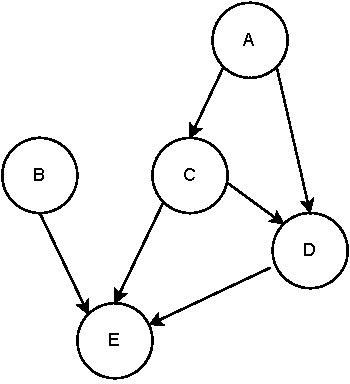
\includegraphics[width=.3\textwidth]{img/dag}
		\caption{orientovaný acyklický graf}
		\label{fig:dag}
	\end{figure}

	Algoritmus při spuštění projde přes celý graf a uloží si do fronty všechny vrcholy, které mají vstupní stupeň nula a následně inicializuje pole pro topologicky seřazené vrcholy. Po úvodní části algoritmus vždy vezme vrchol z fronty, odstraní všechny výstupní hrany, které vycházejí z daného vrcholu. Při odstraňování hrany je kontrolováno zda vrchol, který byl před odstraněním hrany propojen s kontrolovaným vrcholem, nenabývá vstupního stupně nula, pokud ano, vrchol je vložen do fronty. Po odstranění všech výstupní hran daného vrcholu je vrchol vložen na první prázdné místo v poli určené pro výsledný topologicky seřazený graf. Celá smyčka se opakuje dokud není prázdná fronta. Na obrázku \ref{fig:kahn} je ukázán průběh algoritmu. Indegree znázorňuje vstupní stupeň vrcholu.
	
	\newpage
	
	\begin{figure}[h]
		\centering
		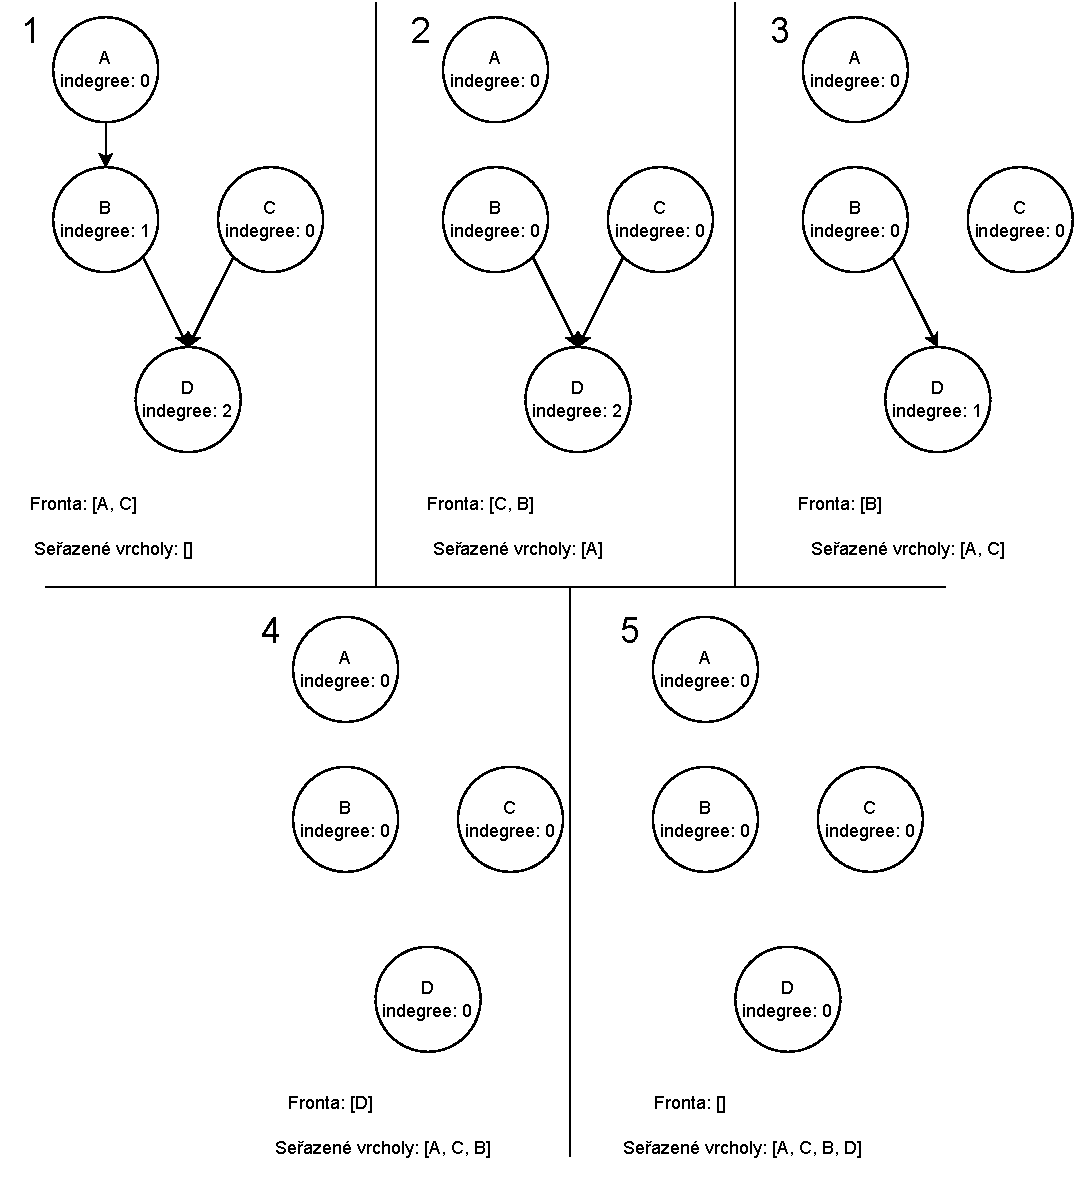
\includegraphics[width=.9\textwidth]{img/kahn}
		\caption{Ukázka Kahnova algoritmu}
		\label{fig:kahn}
	\end{figure}


\newpage

\section*{Pseoudokód Kahnova algoritmu}
	\begin{algorithm}[h]
		\caption{Kahnův Algoritmus pro topologické řazení}
		\begin{algorithmic}[1]
			\Procedure{TopologicalSort}{$G$}
			\State \textbf{Input:} orientovaný acyklický graf $G$
			\State \textbf{Output:} List $L$ (topologicky seřazené vrcholy grafu)
			
			\State Inicializace prázdného listu $L$
			\State Inicializace fronty $S$, který bude obsahovat vrcholy se vstupním stupněm 0
			
			\For{each vrchol $v$ in $G$}
			\If{vstupní stupeň vrcholu $v$ == 0}
			\State Vlož $v$ do $S$
			\EndIf
			\EndFor
			
			\While{$S$ is not empty}
			\State Odstraň vrchol $n$ z $S$
			
			
			\For{each soused $m$ of $n$}
			\State Odstraň hranu mezi $m$ a $n$
			\If{vstupní stupeň vrcholu $m$ == 0}
			\State Vlož $m$ do $S$
			\EndIf
			\EndFor
			\State Vlož $n$ do $L$
			\EndWhile
			
			\If{$L$ obsahuje všechny vrcholy $G$}
			\State \textbf{return} $L$ \Comment{ $L$ je topologicky seřazený graf}
			\Else
			\State \textbf{return} "Graf není acyklický"
			\EndIf
			\EndProcedure
		\end{algorithmic}
	\end{algorithm}

\section*{Experimenty a výsledky}
	
	Prezentovaný algoritmus byl pro účel testování implementován mnou v pythonu. Vlastní implementace byla porovnána s již existující knihovnou Graphlib \cite{r5}. Obě řazení vždy dostanou stejný graf, který bude vždy předem vygenerován. Graf s určitým počtem vrcholů je vždy generován s určitou pravděpodobnostní toho že z vrcholu povede hrana tzn. že čím větší pravděpodobnost tím více bude graf zahuštěn. Pro testování byla zvolena pravděpodobnost 0.2 a 0.6. V tabulce \ref*{tab:tp-sort} jsou výsledky testování a na obrázku \ref{fig:tp-sort} jsou zobrazena data z tabulky v grafu.
	
	\begin{table}[htbp]
		\centering
		\begin{tabular}{c|c|c|c}
			\hline
			Implementace & Počet vrcholů & Pravděpodobnost výskytu hran & Čas řazení, s\\
			\hline
			Gaphlib & 160 & 0.2 & 0.0019\\
			Kahn & 160 & 0.2 & 0.0010\\
			Gaphlib & 160 & 0.6 & 0.0029\\
			Kahn & 160 & 0.6 & 0.0029\\
			\hline
			Gaphlib & 320 & 0.2 & 0.0040\\
			Kahn & 320 & 0.2 & 0.0040\\
			Gaphlib & 320 & 0.6 & 0.0129\\
			Kahn & 320 & 0.6 & 0.0100\\
			\hline
			Gaphlib & 640 & 0.2 & 0.0190\\
			Kahn & 640 & 0.2 & 0.0150\\
			Gaphlib & 640 & 0.6 & 0.0529\\
			Kahn & 640 & 0.6 & 0.0419\\
			\hline
			Gaphlib & 1280 & 0.2 & 0.0820\\
			Kahn & 1280 & 0.2 & 0.0609\\
			Gaphlib & 1280 & 0.6 & 0.2119\\
			Kahn & 1280 & 0.6 & 0.1739\\
			\hline
			Gaphlib & 2560 & 0.2 & 0.2950\\
			Kahn & 2560 & 0.2 & 0.2740\\
			Gaphlib & 2560 & 0.6 & 0.8949\\
			Kahn & 2560 & 0.6 & 0.6956\\
			\hline
			Gaphlib & 5120 & 0.2 & 1.1670\\
			Kahn & 5120 & 0.2 & 1.1130\\
			Gaphlib & 5120 & 0.6 & 3.3829\\
			Kahn & 5120 & 0.6 & 3.0150\\
			\hline
			Gaphlib & 10240 & 0.2 & 5.0363\\
			Kahn & 10240 & 0.2 & 5.2941\\
			Gaphlib & 10240 & 0.6 & 14.5039\\
			Kahn & 10240 & 0.6 & 15.4444\\
			\hline
			Gaphlib & 20480 & 0.2 & 21.0900\\
			Kahn & 20480 & 0.2 & 21.6754\\
			Gaphlib & 20480 & 0.6 & 59.6032\\
			Kahn & 20480 & 0.6 & 104.8810\\
		\end{tabular}
		\caption{Porovnání implementací topologického řazení.}
		\label{tab:tp-sort}
	\end{table}

\newpage

\begin{figure}[htbp]
	\centering
	\begin{tikzpicture}
		\begin{axis}[
			xlabel={Počet vrcholů},
			ylabel={Čas řazení, s},
			legend pos=north west,
			grid=both,
			width=1\textwidth,
			xtick={1000, 5000, 10000, 20000},
			]
			
			\addplot [mark=triangle, blue] coordinates {(160, 0.0019) (320,0.0040) (640,0.0190) (1280,0.0820) (2560,0.2950) (5120,1.1670) (10240,5.0363) (20480,21.0900)};
			\addlegendentry{Gaphlib, 0.2}
			
			\addplot [mark=triangle, green] coordinates {(160, 0.0010) (320,0.0040) (640,0.0150) (1280,0.0609) (2560,0.2740) (5120,1.1130) (10240,5.2941) (20480,21.6754)};
			\addlegendentry{Kahn, 0.2}
			
			\addplot [mark=square, red] coordinates {(160, 0.0029) (320,0.0129) (640,0.0529) (1280,0.2119) (2560,0.8949) (5120,3.3829) (10240,14.5039) (20480,59.6032)};
			\addlegendentry{Gaphlib, 0.6}
			
			\addplot [mark=square, black] coordinates {(160, 0.0029) (320,0.0100) (640,0.0419) (1280,0.1739) (2560,0.6956) (5120,3.0150) (10240,15.4444) (20480,104.8810)};
			\addlegendentry{Kahn, 0.6}
			
		\end{axis}
	\end{tikzpicture}
	\caption{Porovnání implementací topologického řazení.}
	\label{fig:tp-sort}
\end{figure}

Z výsledků je vidět že pro malé grafy (počet vrcholů přibližně 2 - 5000) je implementovaný Kahnův algoritmus zanedbatelně rychlejší v obou různě zahuštěných grafech, ale u větších grafů je implementovaný algoritmus o proti knihovně Graphlib pomalejší a to hlavně u více zahuštěného grafu. 

\newpage
\section*{Závěr}

	Implementovaný Kahnův algoritmus je při malých velikostech grafu zanedbatelně rychlejší než topologické řazení z knihovny Graphlib. Při větších velikostech grafu a malé hustotě je Kahnův algoritmus o něco pomalejší než Graphlib a při zvýšení hustoty grafu se rozdíl mezi rychlosti ještě zvětšuje. Pozitivní aspekty navrhované implementace jsou: jednoduchá implementace, při malých velikostech grafu je implementace rychlejší a při velikých velikostech grafu s nízkou hustotou je podobně rychlá jako funkce z knihovny Graphlib, ale tato implementace Kahnova algoritmu  není vhodná pro veliké grafy s vysokou hustotou.

\bibliographystyle{plain}
\bibliography{bibfile}

\end{document}